\documentclass[11pt, abstract=on]{scrartcl}
\usepackage[formal]{tengwarscript}
\pdfmapfile{=tengwarscript.map}
\usepackage{amsmath,amssymb,amsfonts}
\usepackage{algorithmic}
\usepackage[utf8]{inputenc}
\usepackage[T1]{fontenc}
\usepackage[ngerman]{babel}

\usepackage{hyperref}
\usepackage{graphicx} 

\usepackage{listings}

\def\BibTeX{{\rm B\kern-.05em{\sc i\kern-.025em b}\kern-.08em
    T\kern-.1667em\lower.7ex\hbox{E}\kern-.125emX}}

\begin{document}
\lstset{language=[11]C++}   

\section{Einführung und Allgemeines}
In diesem Praktikum sollten verschiedene parallele Zugriffsmuster auf Grafikarten gemessen und verglichen werden. Dabei verwendet wurde CUDA~\cite{CUDA}, eine von Nvidia entwickelte C++-Erweiterung, die Grafikkarten dieser Firma für parallelisierbare Berechnungen abseits von klassischem Rendering nutzbar macht. In diesem Fall verwendet wurde eine GTX~1070. Einige relevanten Spezifikationen dieser GPU sind:
\begin{itemize}
	\item 1920 Cores, wovon ein Warp jeweils 32~Threads umfasst~\cite{GPUSpecs}
	\item Maximale Taktung laut "`nvidia-smi"': 1708 MHz~\cite{GPUSpecs}
	\item Speicherkonfiguration: 8 GB GDDR5~RAM~\cite{GPUSpecs}
	\item Herstellerangabe für den Durchsatz: 256~GB/s~\cite{GPUSpecs}
	\item PCIe~3.0 fähig, in der Messung wurde allerdings nur PCIe 2.0x16 verwendet. Die maximale Kopierrate von PCIe 2.0x16 entspricht 8.0GB/s~\cite{PCIeSpecs}
\end{itemize}


\subsection{Grundsätzliche Beobachtungen zur Kopierrate}
Eine Grundlage der Programmierung mit der CUDA ist das Management der Daten, welche auf der CPU (genannt "`Host"') oder der GPU (genannt "`Client"') liegen, da CPU-Kerne nur bedingt auf den GPU-RAM zugreifen können und umgekehrt. Mithin ist die mit Standard-Kopieroperatoren erzielbare Kopierrate interessant, die gleichzeitigen einen guten Vergleichsmaßstab für die Effizienz der Verschiedenen Kernel darstellt. Abbildung~\ref{fig:Kopierrate} zeigt die für \texttt{cudaMemcpy()} gemessenen Kopierraten und die vom Hersteller angegebenen Maximalwerte sowie die Spezifikation für den verwendeten PCIe.

\begin{figure} [htbp]
 	\centering
 		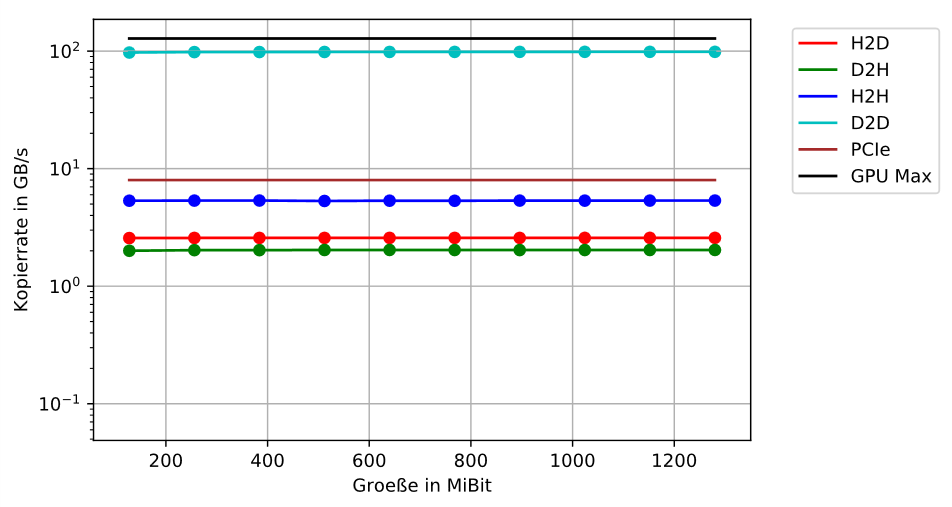
\includegraphics[width=0.7\textwidth]{Graph_Kopierrate.png}
 	\caption{Kopierrate von \texttt{cudaMemcpy()}}
 	\label{fig:Kopierrate}
\end{figure}

Bei der tatsächlichen Durchführungen der Messungen ist es außerdem wichtig, zu beachten, dass jeweils der erste Kernel Aufruf eines CUDA Programms eine wesentlich längere Zeit benötigt als darauf folgende Aufrufe des selben Kernels. Abbildung~\ref{fig:StartupCost} zeigt eine Beispielmessung für einen Empty Kernel, dh. einen Kernel, der zwar aufgerufen wird, dann auf der GPU allerdings keine Arbeit verrichtet. Um dieser Verzerrung entgegenzuwirken, muss vor jeder Laufzeitmessung für einen Kernel dieser einmal als "`Warmup"' aufgerufen, aber dann aus der eigentlichen Messung herausgerechnet werden.

\begin{figure} [htbp]
 	\centering
 		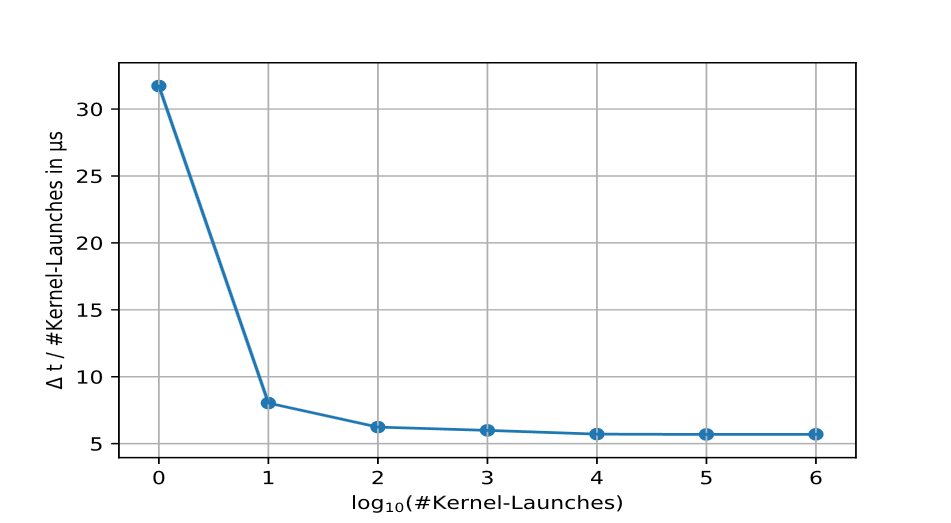
\includegraphics[width=0.7\textwidth]{Graph_Startup.png}
 	\caption{Startup Cost eines Empty Kerneles}
 	\label{fig:StartupCost}
\end{figure}

\section{Copy Kernel} \label{CopyKernel}

Der "`Copy Kernel"', der jeweils ein Element eines Buffers in die entsprechende Position eines anderen Buffers kopiert, lässt sich durch folgenden CUDA-Quellcode beschreiben:

\begin{lstlisting} 
template<typename T>
__global__
void copyKernel(T* out, T* in) {
	unsigned id = threadIdx.x + blockIdx.x * blockDim.x;
		
	out[id] = in[id];
}
\end{lstlisting}

Obwohl die Funktion als Input nur Zeiger auf ein Quell-und ein Ziel-Buffer nimmt, gibt es doch drei implizite Parameter. Diese treten auch bei allen folgenden Messungen auf:
\begin{enumerate}
	\item Anzahl der Blöcke, in die die einzelnen Threads von der GPU gruppiert werden
	\item Die Größe dieser Blöcke
	\item Zugriffstyp \texttt{T} (zB. \texttt{char}, \texttt{int})
\end{enumerate}
 Abbildung~\ref{fig:CopyKernel1} und Abbildung~\ref{fig:CopyKernelBlocks} zeigen die Auswirkungen von Variationen über die drei Parameter auf die durch den Copy Kernel erzielte Kopierrate. Dabei zeigt sich, dass sowohl für die Anzahl der Blöcke, für die Blockgröße als auch für \texttt{sizeof(T)} ein jeweils höherer Parameter zu einer besseren Kopierrate führt. Für hinreichend hohe Werte wird eine Sättigung nahe des Ergebnisses aus Abbildung~\ref{fig:Kopierrate} erzielt. Interessant ist außerdem, dass die Abbildungen sich mit steigendem \texttt{sizeof(T)} je linearer verhalten, je geringer Blockgröße bzw. Blockanzahl sind.

\begin{figure} [htbp]
 	\centering
 		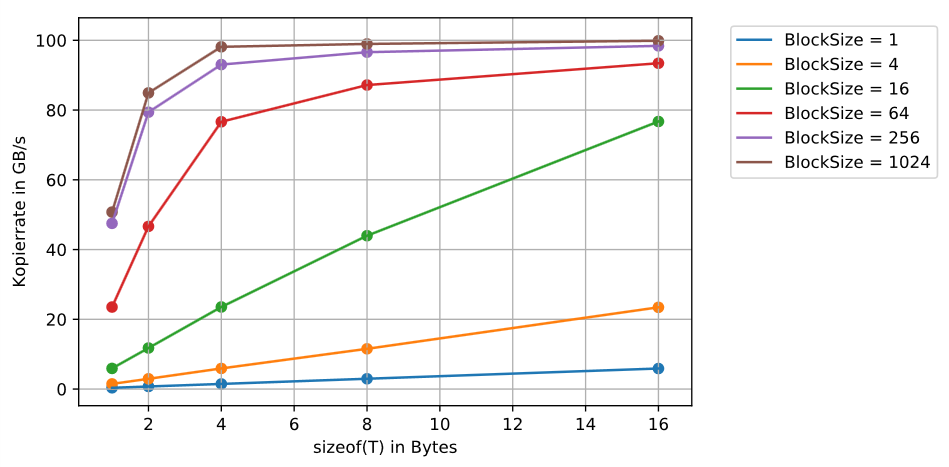
\includegraphics[width=0.7\textwidth]{Graph_CopyKernel1.png}
 	\caption{Variation über \texttt{BlockSize} und \texttt{sizeof(T)}, $\texttt{numBlocks} = 16384$}
 	\label{fig:CopyKernel1}
\end{figure}

\begin{figure} [htbp]
 	\centering
 		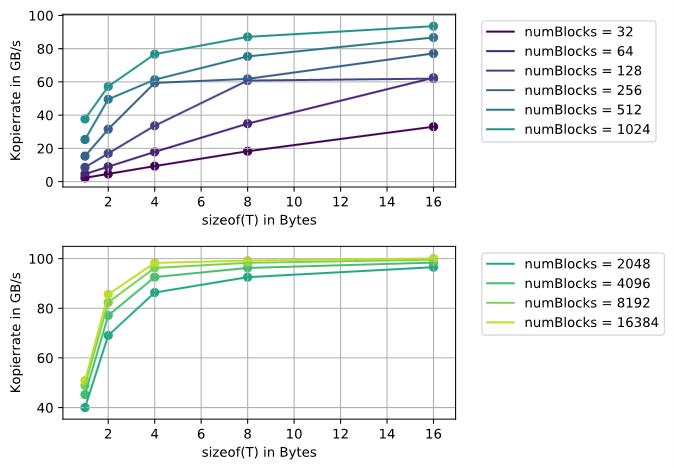
\includegraphics[width=0.7\textwidth]{Graph_CopyKernelBlocks.png}
 	\caption{Variation über \texttt{numBlocks} und \texttt{sizeof(T)}, $\texttt{BlockSize} = 1024$}
 	\label{fig:CopyKernelBlocks}
\end{figure}

\section{Strided Access}
Der Strided Access ist wie folgt definiert:

\begin{lstlisting} 
template<typename T>
__global__
void copyKernel(T* out, T* in, int stride) {
	unsigned id = threadIdx.x + blockIdx.x * blockDim.x;
		
	out[id*stride] = in[id*stride];
}
\end{lstlisting}

Das heißt, der Zugriff erfolgt nicht mehr auf jedes Element konsekutiv hintereinander, sondern nur auf jedes $N$-te Element. Zusätzlicher Parameter ist dann der \texttt{stride}, der festlegt, wie viele Buffer-Einträge übersprungen werden. Bei elementarem Zugriff, wie er zum Beispiel in einer Turingmaschine definiert ist, sollte sich keine Änderung der Kopierrate ergeben, sofern die nicht bearbeiteten Elemente nicht mitgerechnet werden. Beim der Messung zeigt sich aber, dass deutliche Cashe-Effekte auftreten. Bei Messungen zeigt sich ein nahezu exponentieller Abfall der Kopierrate mit steigendem \texttt{stride}, für den die beiden Messungen Abbildung~\ref{fig:StridedAccess1} und Abbildung~\ref{fig:StridedAccess2} beispielhaft stehen. Bei $\texttt{sizeof(T)} \cdot \texttt{stride} = 32$ und $\texttt{sizeof(T)} \cdot \texttt{stride} = 64$ ergeben sich jeweils zwei fast gleiche Werte, und ab $\texttt{sizeof(T)} \cdot \texttt{stride} = 2048$ fällt die Kopierrate wenn überhaupt nur noch vernachlässigbar ab (bei diesen beiden Messungen wie auch bei allen anderen).

\begin{figure} [htbp]
 	\centering
 		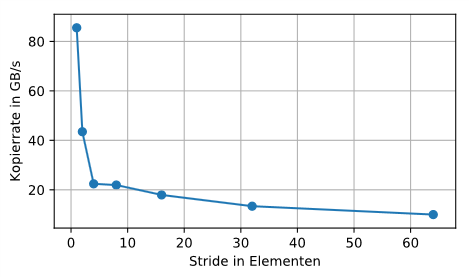
\includegraphics[width=0.7\textwidth]{Graph_StridedAccess1.png}
 	\caption{Strided Access: Variation über \texttt{stride}, $\texttt{BlockSize} = 256$, $\texttt{numBlocks} = 4096$, \texttt{T}:~\texttt{int2}~($\texttt{sizeof(int2)} = 8$)}
 	\label{fig:StridedAccess1}
\end{figure}

\begin{figure} [htbp]
 	\centering
 		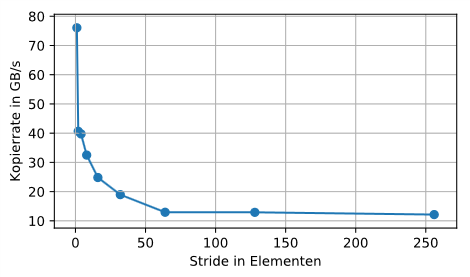
\includegraphics[width=0.7\textwidth]{Graph_StridedAccess2.png}
 	 	\caption{Strided Access: Variation über \texttt{stride}, $\texttt{BlockSize} = 128$, $\texttt{numBlocks} = 2048$, \texttt{T}:~\texttt{int4}~($\texttt{sizeof(int4)} = 16$)}
 	\label{fig:StridedAccess2}
\end{figure}

\section{Offset Access}

Der Offset Access ist ein etwas komplexerer Kernel. Sein Quellcode lautet wie folgt:

\begin{lstlisting} 
template<typename T>
__global__
void oftKernel (T* out,
		T* in,
		const unsigned int sd_size,
		const unsigned int block_size,
		const unsigned int I,
		const unsigned int L)
{
	const unsigned int sd_id = static_cast<int> (threadIdx.x / L);
	const unsigned int id = threadIdx.x - sd_id * L;
	const unsigned int sd_start = blockIdx.x *
			blockDim.x * I + sd_id * L * I;
	
	for (unsigned int i = 0; i < I; i++)
	{
		const unsigned el_id = sd_start + i * L + id;
		((T*) out)[el_id] = ((T*) in)[el_id];
	}
}
\end{lstlisting}

Abbildung~\ref{fig:OffsetZugriff} zeigt das Zugriffsmuster, das aus diesem Kernel resultiert. Ein "`oftKernel"' greift nicht konsekutiv mit jedem Thread auf ein Element der Buffer zu. Er teilt die Buffer zwar in gleich große Abschnitte auf, die jeweils einem Block zugeordnet werden, unterteilt die Blöcke allerdings erneut in Subdomains. Diese Subdomains bestehen dann aus einem gewissen Anteil Threads, die jeweils eine gewisse Anzahl an Iterationen durchführen müssen, um alle Kopiereinträge abzuarbeiten. Neben den bekannten Parametern \texttt{T} und \texttt{BlockSize} ergeben sich dann noch zusätzlich die Anzahl der Iterationen \texttt{I} und die Anzahl der Threads pro Subdomain \texttt{L}. Die Anzahl der Blöcke ergibt sich dann aus diesen Parametern und der Größe der Subdomains auf den Buffern \texttt{sd\_size}.

\begin{figure} [htbp]
 	\centering
 		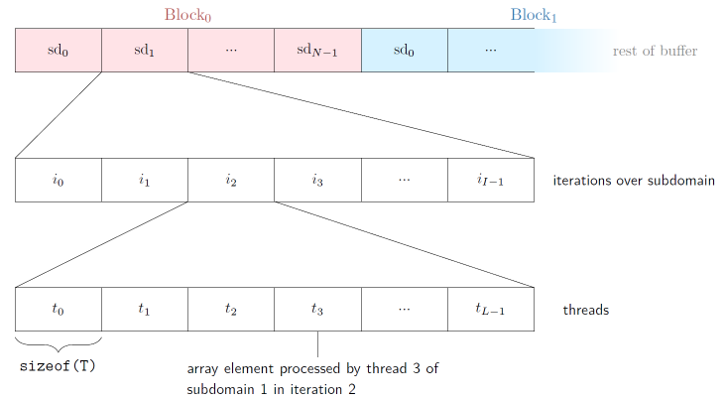
\includegraphics[width=1.0\textwidth]{Graph_OffsetAccessZugriff.png}
 	\caption{Zugriffsmuster des Offset Access}
 	\label{fig:OffsetZugriff}
\end{figure}

\begin{figure} [htbp]
 	\centering
 		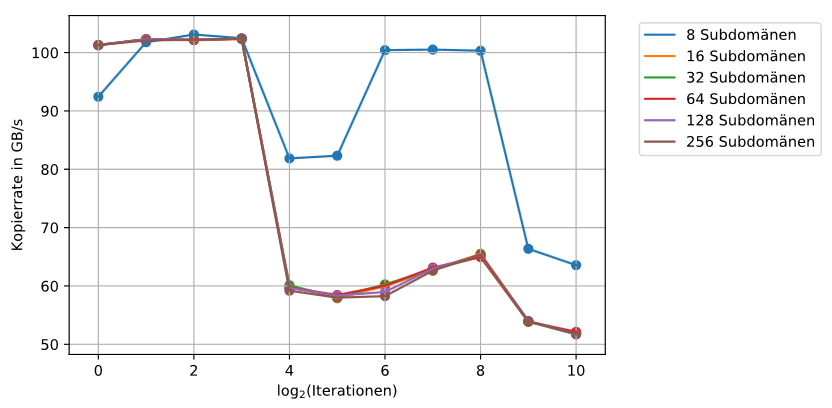
\includegraphics[width=0.7\textwidth]{Graph_OffsetAccessSDpBlock2.png}
 	\caption{}
 	\label{fig:OffsetSD1}
\end{figure}

Die Abbildungen~\ref{fig:OffsetSD1},~\ref{fig:OffsetSD2} und~\ref{fig:OffsetSD3} zeigen verschiedene Variationen über die Parameter des Kernels. Es zeigt sich, dass die Zusammenhänge im Detail komplex sind, und ohne eine tiefere Analyse der verschiedenen Caches der verwendeten GPU (isb. Gesamt-und Zugriffsgröße) wohl nicht vollständig zu verstehen sind. Dennoch lässt sich festhalten, dass eine Sättigung vergleichbar mit vorherigen Kopieroperationen erreicht werden kann, wenn die Parameter richtig gewählt werden, obwohl der Warp, d.h. die jeweils 32 immer gleich ausgeführten Threads, nicht auf nacheinander liegende Elemente zugreifen muss (siehe isb. Abbildung~\ref{fig:OffsetSD3}). Gleichzeitig zeigt sich ein deutlicher Zusammenhang mit der \texttt{L2}-Cache Line-Size von 128 Byte - ist die Zugriffsgröße einer Iteration gleich 128 Byte oder ein ganzzahliger Teiler davon, ist die Kopierrate wesentlich höher.

\begin{figure} [htbp]
 	\centering
 		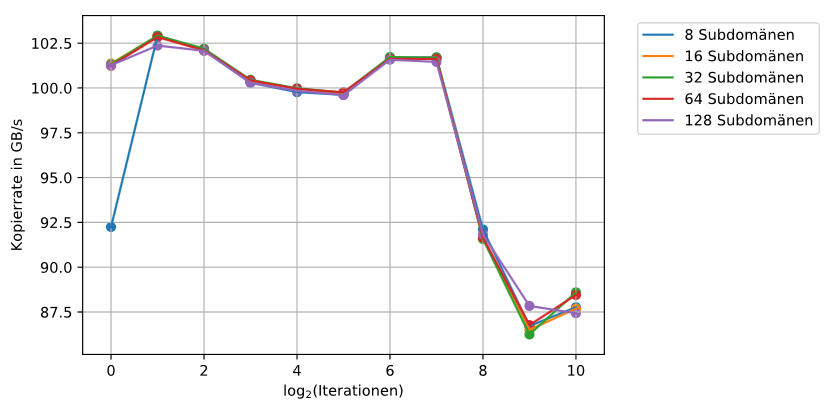
\includegraphics[width=0.7\textwidth]{Graph_OffsetAccessSDpBlock3.png}
 	\caption{}
 	\label{fig:OffsetSD2}
\end{figure}

\begin{figure} [htbp]
 	\centering
 		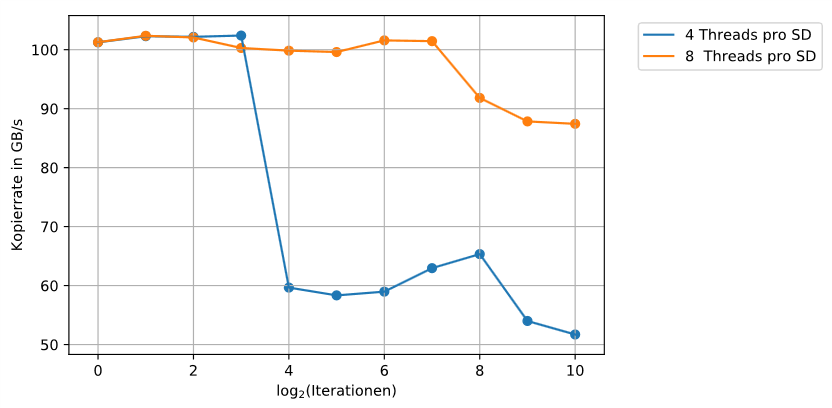
\includegraphics[width=0.7\textwidth]{Graph_OffsetAccessSDpBlock4.png}
 	\caption{}
 	\label{fig:OffsetSD3}
\end{figure}

\section{Allokation: Standard und UnifiedMemory}
Neben der Standard-Allokation über die C++ Funktion \texttt{malloc()} kann CUDA auch mit \texttt{cudaMallocHost()} einen sogenannten Pinned Memory Buffer auf dem Host-RAM allokieren. Dieser erlaubt schnelleres Kopieren und direkte Zugriffe der Kernel auf den Host-RAM, ohne vorher im Code händisch eine Kopieroperation auf den GPU-Speicher vornehmen zu müssen. Mit einem Copy Kernel wie dem aus Kapitel~\ref{CopyKernel} kann dann wieder eine Kopierraten-Messung vorgenommen werden (Abbildung~\ref{fig:CudaMalloc}). Einen Unterschied bezüglich der Anzahl Blöcke scheint es nicht zu geben, die Kurven liegen perfekt aufeinander. Die Kopierrate scheint linear zu steigen, bis eine Sättigung erreicht wird, die etwas unter dem Niveau des Geschwindigkeit des verwendeten PCIe's liegt. Diese Sättigung wird beim Kopieren vom Device zum Host bereits mit weniger Threads erreicht, und das erreichte Niveau ist ein wenig höher. 

\begin{figure} [htbp]
 	\centering
 		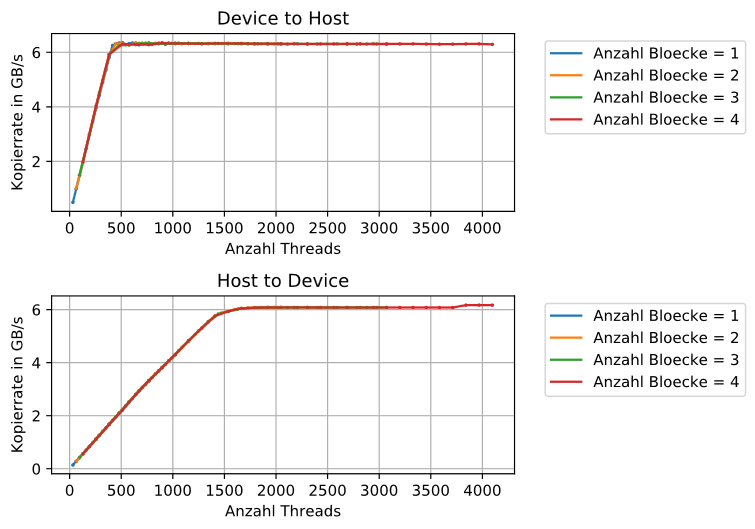
\includegraphics[width=0.7\textwidth]{Graph_CudaMalloc.png}
 	\caption{Copy Kernel Kopierrate auf Pinned Memory, \texttt{T}: \texttt{int}}
 	\label{fig:CudaMalloc}
\end{figure}

Zusätzlich können Buffer in CUDA auch mithilfe von \texttt{CudaMallocManaged()} allokiert werden. Dabei wird vom Programmierer überhaupt keine Angabe getroffen, ob der Buffer auf dem CPU- oder GPU-Ram liegt, sondern CUDA wickelt eventuell benötigte Kopiervorgänge automatisch ab. Abbildung~\ref{fig:CudaMallocManaged} zeigt eine Kopierraten-Messung des Copy-Kernels auf Unified Memory. Dabei wurde durch Cs \texttt{memset()} und CUDAs \texttt{cudaMemset()} sichergestellt, dass die Input- und Output-Buffer jeweils vollständig auf den Host bzw. dem Device RAM kopiert wurden, bevor die Messung begann. Es zeigt sich ein ähnlicher Verlauf wie in der vorherigen Messung, allerdings ist die Form der Kurven viel ungleichmäßiger (möglicherweise ist der Messfehler größer), die Anzahl der Blöcke macht einen deutlicheren Unterschied und die Sättigung wird auch später erreicht.

\begin{figure} [htbp]
 	\centering
 		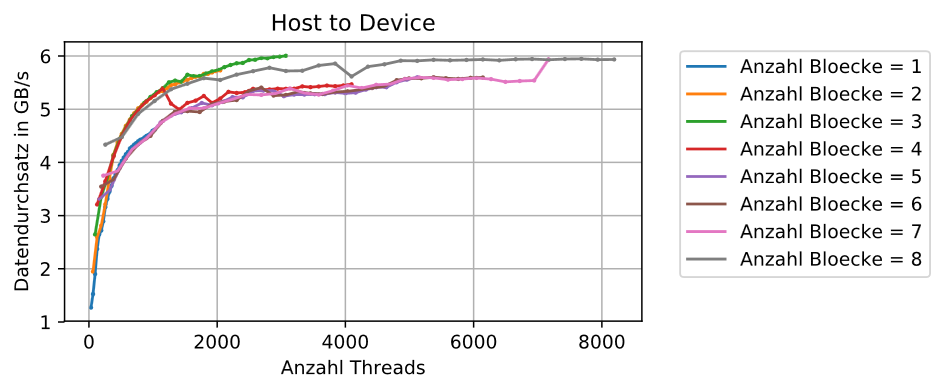
\includegraphics[width=0.7\textwidth]{Graph_CudaMallocManaged.png}
 	\caption{Copy Kernel Kopierrate auf Unified Memory, \texttt{T}: \texttt{int}}
 	\label{fig:CudaMallocManaged}
\end{figure}


\section{Kernel im Producer-Consumer-Verhältnis}
Für diese Messungen wurden zwei identische Grafikkarten benötigt .Aufgrund der Komplexität des verwendeten Codes sei dessen Gestalt hier nur kurz umrissen: Zwei Kernel, die (in eine Richtung) miteinander kommunizieren müssen, d.h. der eine Kernel benötigt für die Erfüllung seiner Aufgabe die Ergebnisse des anderen aber nicht umgekehrt, stehen in einem Producer-Consumer-Verhältnis. Im vorliegenden Fall errechnet dabei der Producer den Durchschnitt eines Teils des Input-Buffers, während der Consumer diesen berechneten Durchschnitt ausliest und ihn vielfach in den entsprechenden Teil gleicher Größe des Output-Buffers dupliziert. Dabei wartet der Consumer jeweils nur auf einen Teil des Buffers, bevor er diesen dupliziert. Eine Grafikkarte führt dann jeweils einen Kernel aus.
Eine Zeitmessung für das Producer-Consumer-System bei Ignorieren der Kommunikation findet sich in Abbildung~\ref{fig:KommunikationOhne}: Die benötigte Zeit steigt also nahezu linear mit den Ergebnissen pro Block, was auch zu erwarten ist, da mit diesen auch die Menge der kopierten Daten steigt.

\begin{figure} [htbp]
 	\centering
 		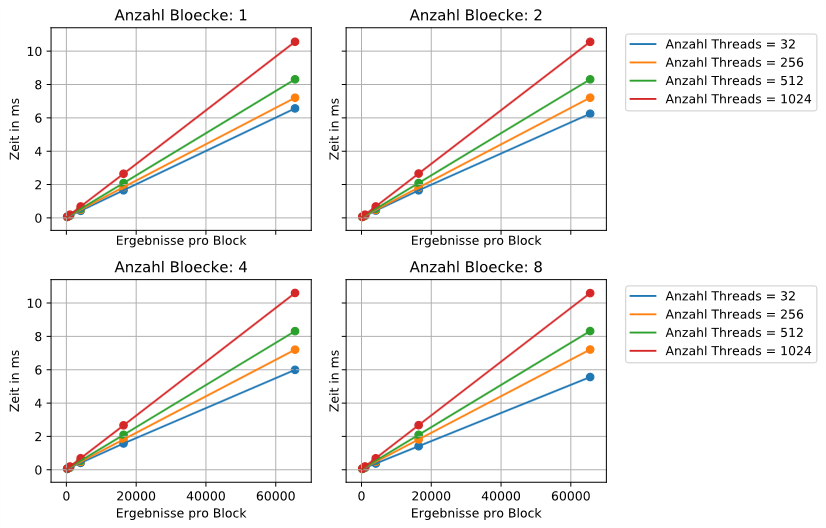
\includegraphics[width=0.7\textwidth]{Graph_KommunikationOhne.png}
 	\caption{Laufzeit Producer-Consumer-Verhältnis ohne Kommunikation}
 	\label{fig:KommunikationOhne}
\end{figure}

Die Graphen mit aktivierter Kommunikation verlaufen ähnlich, allerdings auf einem wesentlich höheren Niveau. Auch die Berechnung des Anteils der Kommunikation am Gesamtergebnis führt demzufolge zu einem mehr oder weniger konstanten Verlauf der Kurven (Abbildung~\ref{fig:KommunikationAnteil}). Lediglich bei einer sehr geringen Anzahl von Ergebnissen pro Block zeigt sich eine gewisse Abweichung. Mit einem Anteil über 80\%, teilweise sogar über 90\% liegt der Kommunikationsanteil jedenfalls sehr hoch, und er scheint mit steigender Anzahl von Blöcken auch leicht zu steigen. Umgekehrt handelt es sich bei dem Ausschlag der Kurve für 8~Blöcke und 1024~Threads beim letzten Wert vermutlich um einen Messfehler.
\begin{figure} [htbp]
 	\centering
 		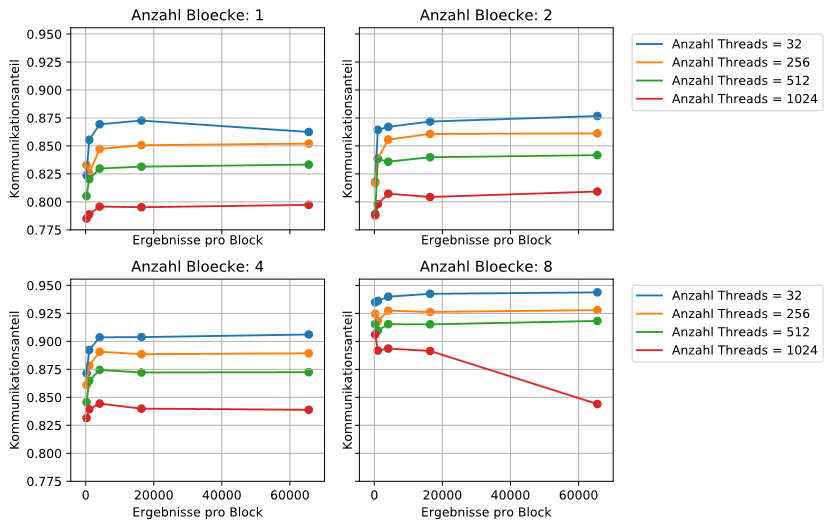
\includegraphics[width=0.7\textwidth]{Graph_KommunikationAnteil.png}
 	\caption{Anteil der durch Kommunikation verlorenen Zeit im Producer-Consumer-Verhältnis}
 	\label{fig:KommunikationAnteil}
\end{figure}

\pagebreak
\begin{thebibliography}{99}
	\bibitem{CUDA}  \href{https://developer.nvidia.com/cuda-zone}{Nvidia Website: ``CUDA Zone'', developer.nvidia.com/cuda-zone}, aufgerufen am 6.2.2019
	\bibitem{GPUSpecs}  \href{https://www.nvidia.com/de-de/geforce/products/10series/geforce-gtx-1070/}{Nvidia Website: ``GTX~1070'', nvidia.com/de-de/geforce/products/10series/geforce-gtx-1070}, aufgerufen am 6.2.2019
	\bibitem{PCIeSpecs}  \href{https://en.wikipedia.org/wiki/PCI_Express}{Wikipedia: ``PCI~Express'', en.wikipedia.org/wiki/PCI\_Express}, aufgerufen am 6.2.2019
\end{thebibliography}
\end{document}

